Le développement du client mobile a suivi le schéma classique de conception d’une application Android. Pour rappel les objectifs initiaux majeurs de ce client étaient de pouvoir récupérer des données sur un web service, les exploiter, les afficher à l’utilisateur et enfin retourner des données au service en question. De façon général la solution Android s’organise en deux projets directeurs : les tests et l’implémentation de l’application.

Il n’a pas été choisi ici de faire du développement dirigé par les tests car la technologie Android était dans le cadre de ce projet une découverte et il aurait était hasardeux de définir des tests Java sur les concepts Android. Les tests ont donc ici vocation à valider les mécaniques métiers a posteriori ainsi que le bon fonctionnement et l’intégrité de l’application au fur et à mesure de l’ajout de fonctionnalités. La partie relative aux tests se subdivise en deux autres : les tests unitaires et les tests instrumentés. Les premiers sont plutôt classiques et permettent de tester les mécaniques métiers et de vérifier tout ce qui est mockable, autrement dit simulable. Toutefois, il y a certains aspects dans un programme Android qu’il n’est pas possible de mocker sans enlever l’intérêt du test. Nous parlons ici de fonctionnalités s’appuyant intrinsèquement sur le système Android comme les appels réseaux, le GPS, l’écran, etc. Il est nécessaire dès lors que l’on veut simuler une fonctionnalité Android même basique, de simuler tout un système Android. D’où l’intérêt de la deuxième catégorie de tests : les tests instrumentés. Ceux-ci vont être exécutés sur un émulateur Android directement afin de pouvoir tester dans notre cas les appels réseaux et l’utilisation du GPS.

Le projet de tests est donc un projet annexe venant en soutien au projet principal : celui du développement de l’application Android. L’ensemble doit gérer des données et les afficher, c’est pourquoi un modèle MVC semblait adapté. Le modèle MVC se compose de trois parties en interaction comme c’est visible \ref{mvc}.

\begin{figure}
    \centering
    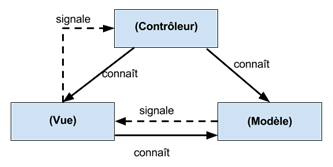
\includegraphics{./img/mvc.png}
    \caption{Patron de conception MVC}
    \label{mvc}
\end{figure}

Le modèle (M) représente les données traitées, dans le cas de l’application ce sont principalement les utilisateurs et leur position GPS. Les deux autres composants n’interagissent pas directement avec les données brutes mais ont accès à l’API du modèle symbolisée par le gestionnaire d’utilisateur (UserManager) comme sur la \ref{model}. Le modèle gère donc tous les petits traitements bas niveau sur les données et les sert au reste de l’architecture selon les besoins.

\begin{figure}
    \centering
    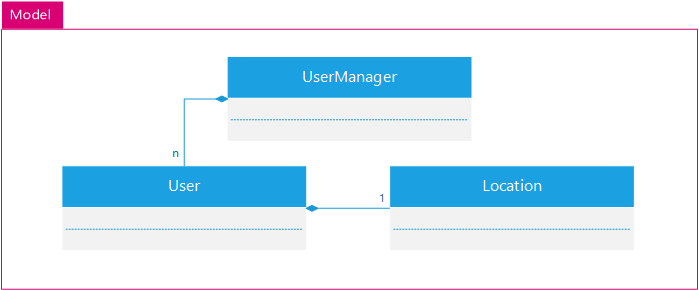
\includegraphics{./img/android-model.png}
    \caption{Diagramme du modèle}
    \label{model}
\end{figure}

Le contrôleur (C) s’occupe des interactions avec l’utilisateur, il doit pouvoir transmettre les commandes émanant de l’utilisateur aux autres composants. Dans le cadre de l’application Android, le contrôleur est symbolisé par les activités : ce sont les activités Android qui proposent les interfaces de contrôle utilisateur. Elles permettent de recevoir les évènements utilisateur comme un clic ou encore les messages du système comme l’arrivée d’un SMS ou encore l’actualisation de la position GPS. Les informations reçues peuvent ensuite être utilisées pour effectuer une mise à jour du modèle ou un rafraîchissement de l’affichage. Les différents types d’activités sont visible sur \ref{controller}.

\begin{figure}
    \centering
    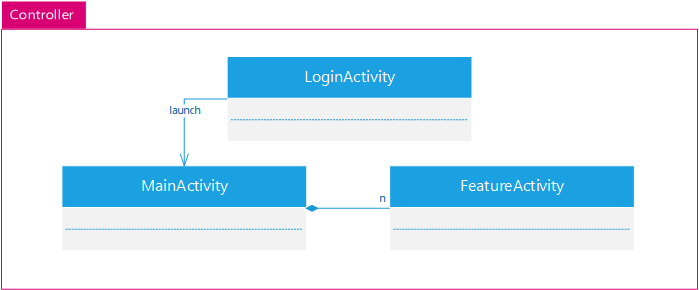
\includegraphics{./img/android-controller.png}
    \caption{Diagramme du contrôleur}
    \label{controller}
\end{figure}


La vue (V) est l’ensemble des éléments constituant la façon dont vont être présentées les données. La réalisation concrète dans l’application Android de la vue est faite par les fichiers XML de layout et autres ressources. Dans la vue entre aussi un pan important du concept de l’application : la gestion de l’affichage 3D. En effet, pour la plupart des éléments d’interface, tout peut être géré par des fichiers de métadonnées mais pour générer la carte en trois dimensions d’un lieu il est nécessaire de décrire dans le code la manière d’utiliser les données pour les afficher avec de véritables classes Java. La vue est donc un ensemble complexe constitué de diverses ressources comme on peut le voir sur \ref{view}.

\begin{figure}
    \centering
    \includegraphics{./img/view-android.png}
    \caption{Diagramme de la vue}
    \label{view}
\end{figure}

Le tout s’interconnecte et interagit donc pour faire fonctionner l’ensemble. Mais pour alimenter l’application en données exploitables, des services ont dû être mis en place. Il en existe deux qui servent de sources de données au programme. Le premier est le service GPS, il permet à l’application de récupérer la position du dispositif Android. Dans un premier temps, ce service été basé uniquement sur les données matérielles de l’appareil mais afin d’améliorer la précision, l’utilisation des Google Services a été choisie. Les Google Services utilisent à la fois les données GPS pures mais aussi leur historique ainsi que les données du gyroscope et de l’accéléromètre pour déterminer la position avec une plus grande précision. Ceci s’est avéré indispensable pour une localisation correcte en intérieur.

Le deuxième service est celui responsable de la communication avec le serveur et qui permet de le requêter. Ainsi ce service permet à la fois d’envoyer sa propre position au serveur mais aussi de récupérer la liste des utilisateurs connectés et leurs informations. Ce service exécute en parallèle du thread principal des requêtes http sur le web service WatchDogZZ. Pour ce faire, il utilise la bibliothèque Volley qui permet d’effectuer simplement des communications sur le réseau.

Le patron de conception majeur dans ce système applicatif est celui observer-observable : il permet à une des entités d’être prévenue par une autre après inscription qu’un traitement a été effectué. Ceci permet le parallélisme des services et de ne pas bloquer l’interface graphique lors d’un traitement long (communication réseau).

L’ensemble est sécurisé par le système d’authentification Google. Ce choix a été motivé par la simplicité puisque le client étant sur un système Android, il possède forcément un compte Google associé. Il suffit alors d’effectuer une requête sur les serveurs de Google avec les informations d’authentification de l’appareil pour récupérer un token validant l’identité de l’utilisateur. Ce token est ensuite transmis lors de chaque requête au serveur WatchDogZZ en vue de vérifier l’identité du demandeur (voir la \ref{token}).

\begin{figure}
    \centering
    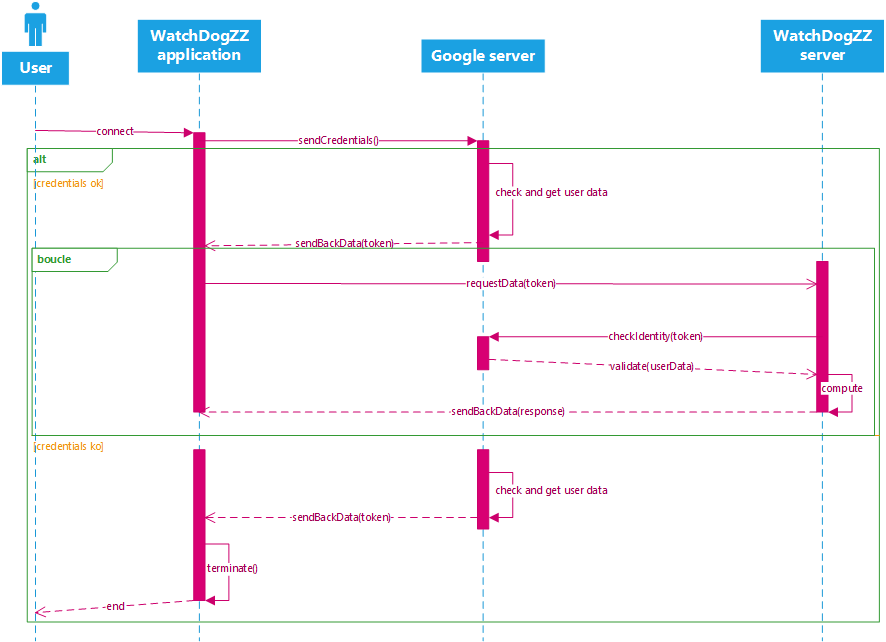
\includegraphics{./img/android-token.png}
    \caption{Utilisation du token Google}
    \label{token}
\end{figure}

La carte du maraudeur est une vue qui a été créée spécialement pour l’application. Elle se base sur une SurfaceView reposant sur de l’OpenGL ES 2. L’intérêt était à la fois de pouvoir dessiner en deux mais aussi trois dimensions. Un Renderer spécial a été implémenté ainsi que des managers de ressources 3D. Il est ainsi possible de gérer cette vue comme un observer du UserManager. La vue pourra par la suite afficher les scènes 3D avec les différents éléments à chaque notification. Les différentes classes entrant en jeu sont visibles sur la figure \ref{3d} ainsi que leur rôle dans le MVC.

\begin{figure}
    \centering
    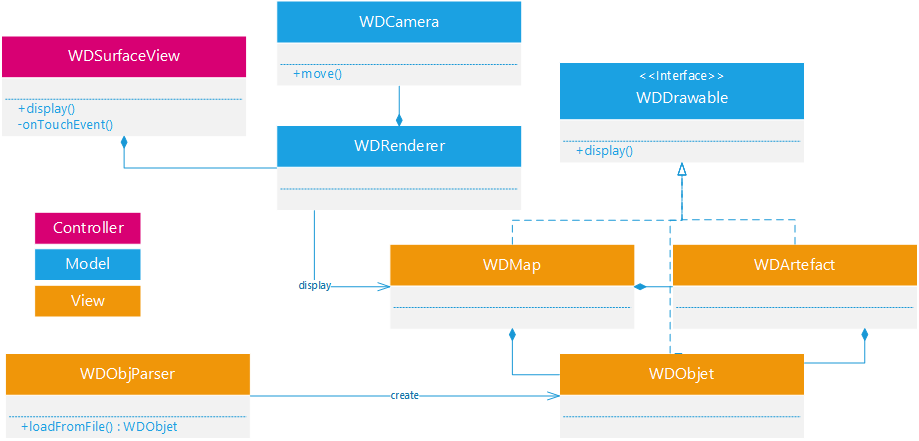
\includegraphics{./img/android-3d.png}
    \caption{Fonctionnement de la 3D Android}
    \label{3d}
\end{figure}

La conception de l’application Android est très simple mais fait intervenir de nombreux éléments et services qui touchent énormément d’aspects de la programmation Android. Il existe sur les versions les plus récentes du Framework des fonctionnalités plus intéressantes et performantes toutefois le choix a été fait d’essayer de faire l’application la plus diffusable possible et donc de supporter un maximum d’appareil. Au début du développement, la version choisie était la 9 mais suite à des contraintes inévitables de développement nous avons dû monter à la version 12. Ceci reste correct d’autant plus que cela représente toujours plus de 99% de parts de marché.




La méthode adoptée pour la conception de cette solution devait pouvoir convenir à un projet hétérogène et à une équipe de taille faible, un binôme. De façon générale le projet se décomposait en trois sous-projets indépendants : la partie serveur, la partie client et la partie documentation.

La partie documentation est la seule qui a réellement fait l’objet d’un travail commun avec concertation, échange de points de vue et vérification du travail de l’autre puisqu’elle a consisté en la mise au point des spécifications et en la rédaction de ce rapport. Durant la phase d’analyse et devant l’état des lieux de tout ce qui devait être fait, il a paru équitable et logique de détaché une personne sur le projet Android et une autre sur le projet serveur. Ainsi la répartition des tâches et l’expertise sur les différents projets étaient très contrôlé.

Une fois que les besoins de l’application ont été analysés et que les spécifications ont été posées, nous avons transformé ses documents en un kanban regroupant les user stories principales. Ces user stories forment l’ensemble minimal des tâches à effectuer pour avoir une application fonctionnelle répondant aux demandes fondamentales du cahier des charges. Dès lors que cette sélection a été faite, le développement des projets primitifs du client et du serveur a commencé. Des échanges réguliers sur les outils de travail d’équipe de GitHub, que nous détaillons plus loin, ont permis de suivre l’évolution du développement linéaire de chaque projet et de rendre compte du travail effectué. L’objectif de cette période était donc de livrer une version fonctionnelle de l’application pour la mi-janvier.

Au terme de cette première période nous avons pu livrer une application répondant aux critères minimaux et permettant de suivre des personnes dans l’ISIMA. En partant de cette base fonctionnelle nous avons commencé le développement de fonctionnalités plus poussées avec une méthode un peu différente : une méthode plus agile.

Nous avons listé tous les bugs connus, les améliorations et les fonctionnalités que nous souhaitions ajouter. Ensuite nous avons commencé à fonctionner en itérations agiles d’une durée de deux semaines. En début d’itérations nous sélectionnions un ensemble d’items qui étaient des « issues » sur GitHub et nous en faisions une milestone. Nous travaillions ensuite sur ces issues et en fin de cycle nous faisions le point sur l’itération terminée et nous rajoutions des issues en fonction de la situation. Le développement agile a permis de rajouter des fonctionnalités avancées sur deux ou trois itérations.

L’ensemble de ces éléments fait que nous avons pu développer étape par étape une application qui semblait très complexe à mettre en place. Sans cette méthode nous aurions peut-être été perdu devant tout le travail mais dans les faits, malgré quelques difficultés nous avions toujours une version fonctionnelle qui répondait aux critères minimaux du cahier des charges.
 
Le travail présenté dans ce rapport concerne l'élaboration d'une solution visant à faciliter l’\textbf{orientation} des usagers au sein d'un bâtiment. Pour ceci, les utilisateurs disposent d'une \textbf{carte interactive} sur \textbf{plateforme mobile} se mettant à jour par des requêtes sur un \textbf{service web} afin d’afficher en temps réel la position des autres usagers ou bien des points d’intérêt. Ce projet s’inspire de la carte du maraudeur de l’univers Harry Potter et se découpe donc en deux parties distinctes : une partie service web, ainsi qu'une partie application mobile \textbf{Android}.

La partie service web est réalisée en utilisant le module \textbf{Express} ajouté au framework de base \textbf{NodeJS}, permettant de réaliser simplement un serveur web. D'autres modules complémentaires viennent s'ajouter pour disposer de plus de fonctionnalités. Ce service permet de traiter des requêtes soumises par les clients mobiles, ainsi que de stocker des données relatives au bon fonctionnement de l'application.

La seconde partie concernant l'application Android permet à un utilisateur d’afficher la carte interactive en se connectant au service web. Cette application effectue des requêtes visant à mettre à jour la position de l'utilisateur sur le service web. Ainsi l’application des autres utilisateurs est capable de récupérer ces \textbf{données ouvertes} et de les placer au sein de leur propre carte modélisant un bâtiment.

Les tests de cette solution ont pu montrer qu'il est possible d'afficher la position des utilisateurs sur une carte modélisée de l'ISIMA. Cependant, des erreurs de positionnement se retrouvent dans la position des utilisateurs, du fait de la mauvaise réception GPS par le mobile. Cette solution mise en place pourra faire l'objet d'améliorations futures telles que l'ajout d'itinéraires entre deux utilisateurs ou vers un point d'intérêt.

%%
Carte interactive, Express, NodeJS, Android, service web, mobile, données ouvertes, maraudeur.
 
\section{Etudes préalables}

Avant de commencer à parler de tout l’aspect technique et conception nous allons resituer notre projet en définissant ses objectifs, son plan de route et ses inspirations.

\subsection{Présentation du projet}

Ce projet a été mis en place de notre propre initiative et nous avons donc défini les objectifs à atteindre ainsi que les fonctionnalités de nous-même, avec l'aide du tuteur de projet.

L’idée originelle que nous avions proposée était inspirée de la carte du Maraudeur de l’univers Harry Potter visible sur la figure \ref{marauder}. Cette carte permet grâce à la magie de suivre en temps réel toutes les personnes présentes à Poudlard, l’école de sorciers, puisque leurs pas apparaissent dessus avec leur nom. Cet objet, bien que magique, nous semblait aujourd’hui pouvoir être réalisé grâce aux avancées liées au domaine des objets connectés. 

\begin{figure}[H]
    \centering
    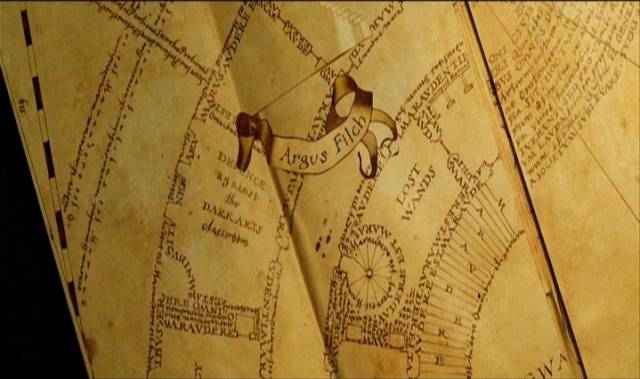
\includegraphics{./img/marauder.jpg}
    \caption{Morceau de la carte du Maraudeur tirée du film}
    \label{marauder}
\end{figure}

Nous avons donc décidé de proposer une manière simple pour tout le monde de pouvoir s'orienter et retrouver des personnes dans les locaux de l'ISIMA au travers d’une application. Cette solution devra donc récolter l’ensemble des données sur les usagers de l’ISIMA et les reporter sur une carte qui sera bien sûr électronique. Nous voulons ainsi que chacun puisse sortir notre carte de sa poche pour retrouver un ami ou un collègue instantanément.

De manière générale, nous devons être capable de visualiser une carte de l'ISIMA, mais également de pouvoir trouver facilement une personne, un bureau ou une salle de cours. De plus, il serait intéressant de pouvoir localiser n'importe quelle autre personne sur la carte en temps réel. Cette visualisation doit s'actualiser assez rapidement pour que la localisation de personnes soit la plus précise possible pour les utilisateurs.

Une fois cette solution éprouvée avec les bâtiments de l'ISIMA, nous pouvons penser l'étendre à n'importe quel autre bâtiment dont nous pouvons avoir les plans. L’intérêt ici étant de développer une preuve de fonctionnement du suivi de personnes dans un bâtiment qui plus est considéré comme étant très surchargé de signaux. Comme nous l’évoquions plus tôt ceci pourrait trouver différentes utilisations dans différents contextes comme par exemple le fonctionnement d’un hôpital, la surveillance d’une prison, l’évacuation d’un bâtiment. Avec l’avènement de l’open data, il y a aussi de nombreuses questions éthiques à résoudre vis-à-vis des informations récoltées et diffusées.


\subsection{Analyse de l'existant}

Nous ne nous attarderons pas dans cette partie sur la carte magique imaginée par J. K. Rowling mais nous allons plutôt voir les différentes applications existant autour de la localisation d’usagers.

Le premier exemple est celui des réseaux sociaux. En effet, avec leur avènement est arrivé aussi un moyen pour des grands groupes de récolter une masse importante d’information sur leurs utilisateurs : ce que l’on appelle le Big Data. Dans cette masse de données, il y a bien évidemment des données de géolocalisation. Celles-ci sont de plusieurs types : soit données, soit mesurées.

Les premières, dites données, sont les informations que l’utilisateur va donner de lui-même aux réseaux sociaux comme par exemple poster une photo d’une après-midi entre amis en spécifiant le lieu de la prise de vue. Cette information peut être légitimement utilisée puisque donnée par l’utilisateur mais cela ne représente pas une source fiable ni même précise. Même si cette information n’est pas fiable, les réseaux sociaux ont trouvé depuis 2014 une toute nouvelle utilisation à ce type d’information : l’aide aux personnes en danger. En effet, Facebook a développé un service nommé Safety Check qui repère les personnes présentes à proximité d’une zone de danger que ce soit une catastrophe naturelle ou bien encore une action terroriste et leur propose de se signaler en sécurité auprès de leurs proches. Le Safety Check visible à la figure \ref{safety-check} est un bon exemple de localisation de personnes mais demande à ce que les personnes recherchées effectuent une action.

\begin{figure}[H]
    \centering
    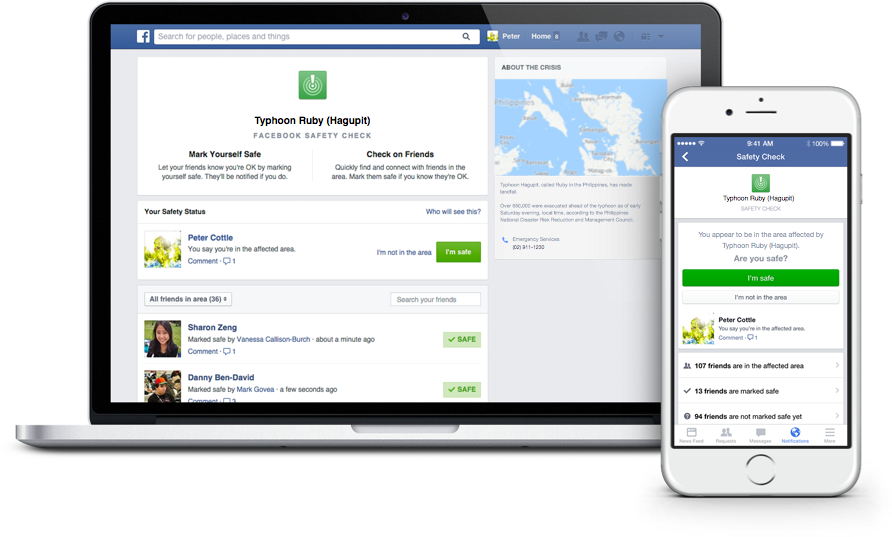
\includegraphics{./img/safety-check.png}
    \caption{Service Safety Check de Facebook}
    \label{safety-check}
\end{figure}

Le second type dit données mesurées représente toutes les informations que les réseaux sociaux récupèrent sur les appareils des utilisateurs. Cette récupération est rendue possible tout d’abord par l’existence de ces données. En effet depuis quelques années avec l’arrivée des smartphones et des objets connectés, la majeure partie des appareils électroniques possèdent des fonctionnalités de géolocalisation. Il est alors facile pour une application d’accéder à la position de son utilisateur. En général, l’appareil en question est un smartphone et se trouve très souvent au même endroit que son propriétaire, voire sur lui-même. On peut clairement constater la récupération de ces informations lorsque la localisation d’un utilisateur est associée directement au message qu’il poste ou bien encore sur les historiques. En effet, Google propose à ses utilisateurs d’accéder à tous l’historique de leurs déplacements comme on peut le voir sur la figure \ref{google-maps}. Google récupère en permanence la position de utilisateurs afin de pouvoir fournir à la communauté des statistiques sur l’affluence de certains lieux, de demander des informations et photos sur les lieux en cours de visite ou bien proposer des services à proximité. Google arrive ici à localiser avec précision dans quel établissement une personne se trouve mais ne partage pas les données individuelles au reste de la communauté.

\begin{figure}[H]
    \centering
    \includegraphics{./img/google-maps.png}
    \caption{Suivi des déplacement sur Google Maps}
    \label{google-maps}
\end{figure}

KHEOLY RENNES

APPLICATION ANDROID

\subsection{Spécifications du projet}

Etant donné que peu de solutions sont disponibles sur le marché, nous avons choisi de partir de zéro et créer notre solution. Cela nous permet également d'avoir un contrôle total sur les données, du projet, les diverses implémentations de fonctionnalités ainsi que la manière dont nous souhaitons utiliser notre solution.

La solution la plus évidente en termes de support de visualisation pour les utilisateurs et de leur proposer une application qu'ils pourront installer sur leur smartphone, pc, montre connectée ou encore tablette.
Afin de rendre cette application dynamique et de proposer un suivi de position d'utilisateurs en temps réel, il est convenu d'utiliser un Service Web. Ce service permettra également de stocker des informations utiles aux utilisateurs, ce qui permettra également d'alléger le volume de données stockées sur leurs terminaux.

\subsubsection{Architecture}

L'architecture choisie pour organiser notre solution est la suivante.

\begin{figure}[H]
    \centering
    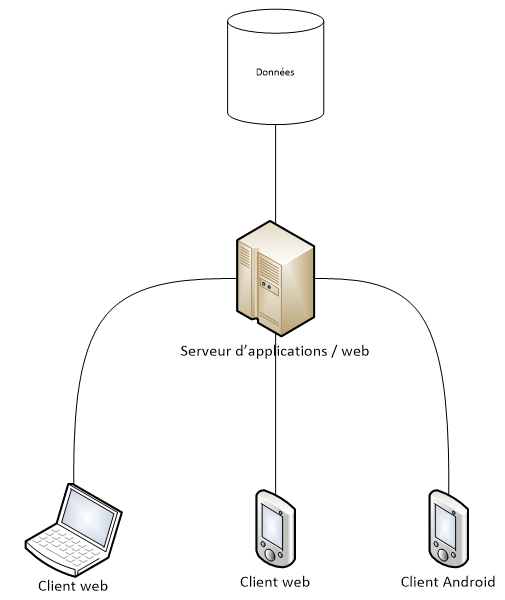
\includegraphics[height=10cm]{../infrastructure.png}
    \caption{Architecture}
    \label{architecture}
\end{figure}

Nous pouvons observer dans la figure~\ref{architecture} que celle-ci ressemble à une architecture client/serveur, ce qui est le but recherché.

\subsubsection{Partie serveur}
La partie centrale est celle du Web Service. Le serveur doit etre capable de répondre aux différentes connexions et requêtes des utilisateurs (se connectant sur l'application Android ou tout autre...). Le serveur sera un Service Web de type \textbf{REST} disposant pour fonctionnalités minimales :
\begin{itemize}
    \item de s'authentifier ;
    \item d'obtenir les positions d'autres personnes connectées sur l'application ;
    \item obtenir la liste des personnes connectées ;
    \item envoyer la position actuelle de l'utilisateur connecté ;
    \item se déconnecter.
\end{itemize}

Ces fonctionnalités seront essentielles pour le fonctionnement de base de l'ensemble de la solution. Par la suite, des fonctionnalités supplémentaires pourront être ajoutées dans l'application, par exemple :
\begin{itemize}
    \item historique des positions ;
    \item calcul d'itinéraire entre 2 positions dans le bâtiment ;
    \item partage de position (par sms, mail, ...).
\end{itemize}

Pour stocker les diverses informations utilisateur (login, position), nous avons convenu d'utiliser une base de données qui s'interfacera directement avec le Service Web.

\subsubsection{Partie Android}
Une seconde partie comporte une application Android (qui pourrait être déclinée pour iOS et Windows Phone). Cette application permettra :
\begin{itemize}
    \item de s'inscrire
    \item de se connecter
    \item envoyer sa position gps au service web
    \item recevoir les positions gps d'autres utilisateurs connectés
    \item visualiser en temps réel sur une carte les positions
\end{itemize}

L'application pourra évoluer et proposer :
\begin{itemize}
    \item la carte en version 3D
    \item la carte en version VR
    \item l'ajout d'informations sur la carte (lieu / point de rdv)
\end{itemize}

Le choix d'une application Android se justifie par :
\begin{itemize}
    \item la communauté Android est active
    \item la quantité de terminaux
    \item l'un de nous a des connaissances en Android
\end{itemize}
La mise à jour des positions est soit faite par l'application qui effectue une requête sur le serveur, soit c'est le serveur qui renvoie les positions des utilisateurs ayant bougé d'un delta suffisant qui permet sa mise à jour chez les utilisateurs. Les frameworks 3.X+ seront supportés pour fonctionner sur un maximum de terminaux.


\subsubsection{Intégration continue}
Un des objectifs de ce projet est de mettre en place une intégration continue et un déploiement automatique. Pour ce faire il est nécessaire d'avoir deux serveurs :
\begin{itemize}
    \item un serveur d'application
    \item un serveur d'intégration
\end{itemize}

Le premier sera certainement un CaaS Amazon pour NodeJS. Le serveur d'intégration sera un serveur Travis CI puisqu'il gère à la fois le NodeJS et l'Android (nouvelle fonctionnalité). Cela permettra contrairement à un serveur Jenkins de déployer facilement sans avoir à gérer un serveur mais juste en utilisant un service.

\subsection{Organisation du travail}

L'organisation temporelle théorique du travail est décrite dans le diagramme de Gantt ci-dessous.

\begin{landscape}
    \begin{figure}[h]
        \centering
        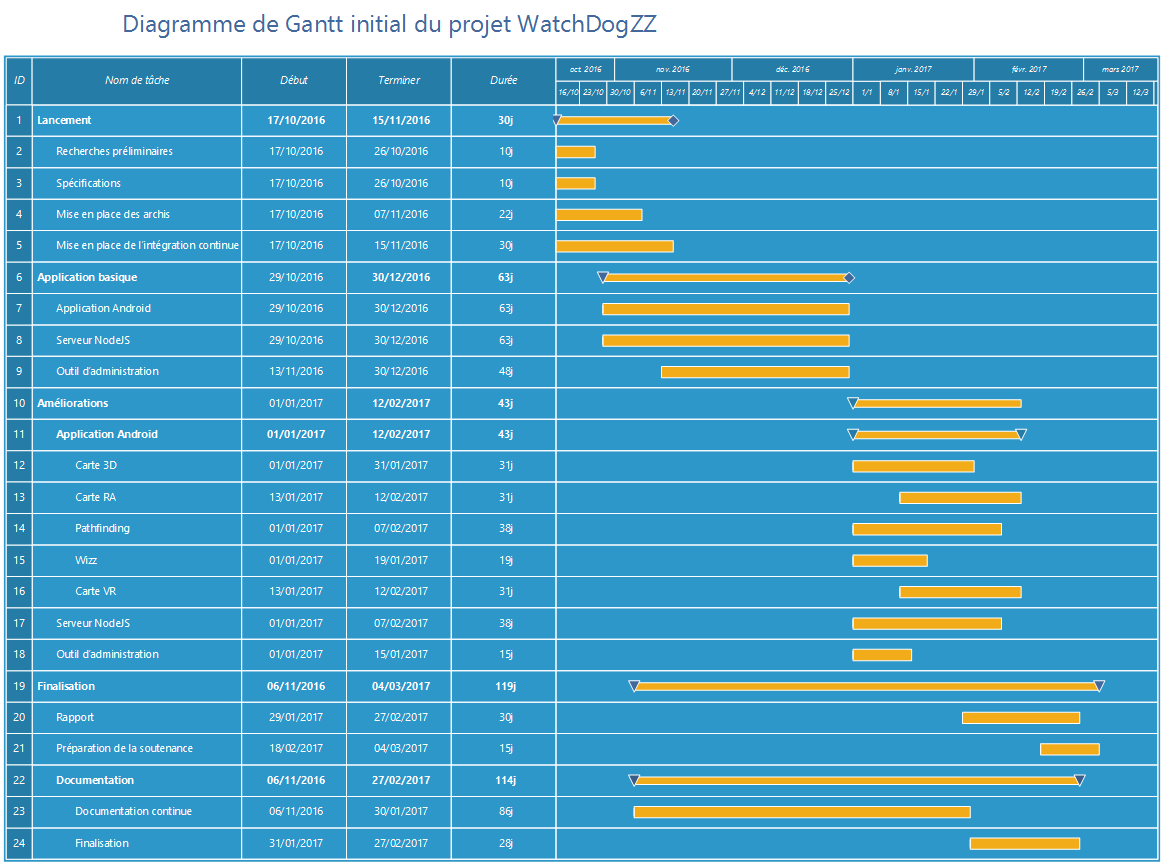
\includegraphics[height=\textwidth]{../gantt_initial.png}
        \caption{Diagramme de Gantt théorique}
    \end{figure}
\end{landscape}

suite...
